\documentclass[11pt,a4paper,openright,twoside]{extreport}
\usepackage[utf8]{inputenc}
\usepackage[english]{babel}
\usepackage[inner=2cm,outer=2cm,top=2cm,bottom=2cm]{geometry}
\usepackage{graphicx}
\usepackage{amsmath}
\usepackage{amsfonts}
\usepackage{textcomp}
\usepackage{amssymb}
\usepackage{pifont}
\usepackage{epstopdf}
\usepackage[singlespacing]{setspace}
\usepackage{tabularx}
\usepackage{arydshln}
\usepackage{mathrsfs}
\usepackage{rotating}
\usepackage{caption}
\usepackage[usenames,dvipsnames]{xcolor}
\usepackage{fancyref}
\usepackage{subcaption}
\usepackage{braket}
\usepackage{color}
\usepackage{float}
\usepackage{enumerate}
\usepackage[pagebackref]{hyperref}
\usepackage{afterpage}
\usepackage[makeroom]{cancel}

\usepackage{fancyhdr}
\pagestyle{fancy}

\usepackage{graphicx}
\usepackage{subcaption}
\usepackage{wrapfig}
\graphicspath{{images/}}

\fancyhead{}
\fancyhead[RE, LO]{{\nouppercase{\rightmark{Dhole, Mensing, Padalkar}}}}
\fancyhead[LE, RO]{\thepage}
\setlength{\headheight}{15pt}
\renewcommand{\headrulewidth}{0.4pt}

\fancyfoot{}
\fancyfoot[RE, LO]{{\nouppercase{\leftmark{MAS-SS2018 | Hochschule Bonn-Rhein-Sieg}}}}
\fancyfoot[LE, RO]{Due Date: 19.04.2018}
\renewcommand{\footrulewidth}{0.4pt}

\hypersetup{
    pdftoolbar=true,        % show Acrobat’s toolbar?
    pdfmenubar=true,        % show Acrobat’s menu?
    pdffitwindow=false,     % window fit to page when opened
    pdfstartview={FitH},    % fits the width of the page to the window
    pdftitle={Scientific Experimentation and Evaluation Homework},    % title
    pdfauthor={Pranjal Dhole},     % author
    pdfsubject={Review},   % subject of the document
    pdfcreator={Pranjal Dhole},   % creator of the document
    pdfproducer={Pranjal Dhole}, % producer of the document
    pdfkeywords={SEEHomework} {Scientific Experimentation and Evaluation}, % list of keywords
    pdfnewwindow=true,      % links in new window
    colorlinks=true,       % false: boxed links; true: colored links
    linkcolor=MidnightBlue, % color of internal links (change box color with linkbordercolor)
    citecolor=Thistle,        % color of links to bibliography
    filecolor=magenta,      % color of file links
    urlcolor=Sepia           % color of external links
}
%%%%%%%%%%%%%%%%%%%%%%%%%%%%%%%%%%%%%%%%%%%%%%%%%%%%%%%%%%%%%%%%%%%%%%%%%%%
%specific
\raggedbottom
%%%%%%%%%%%%%%%%%%%%%%%%%%%%%%%%%%%%%%%%%%%%%%%%%%%%%%%%%%%%%%%%%%%%%%%%%%%
\pagenumbering{arabic}
\begin{document}
%%%%%%%%%%%%%%%%%%%%%%%%%%%%%%%%%%%%%%%%%%%%%%%%%%%%%%%%%%%%%%%%%%%%%%%%%%%
\begin{center}
\section*{\underline{Scientific Experimentation and Evaluation}\\{Assignment 1.1}}
\large{Abhishek Padalkar, Max Mensing, Pranjal Dhole}\\
\large{Due date: Thursday, 19$^{\text{th}}$ April, 2018}
\end{center}

\subsection*{1. Soft tissue measurement experiment: Formalization general terms}
\begin{table}[ht]
\centering
\begin{tabular}{lcl}
Measurand &-& Force \\
Measurement &-& Axial Force\\
Display &-& Digital (NI DAQ) \\
Measurement Range &-& 0.0987N \\
Measured (Quantity) Value &-& Indentation depth (mm)\\
Measurement Result &-& 4.6N \\
Device under Test &-& Force torque (FT) sensor \\
Measurement Facility &-& Indenter \\
Measurement System &-& Indenter + tissue model \\
Meter &-& FT Sensor \\
Measuring Principle &-& linear compression \\
Measuring Method &-& compression in FT sensor's coordinate system \\
Sensitivity &-& Axial Force - 0.04N \\
\end{tabular}
\end{table}

\subsection*{2. Assignment 1.1}
\begin{enumerate}
\item As shown in fig.\ref{legobot}, we use LEDs that are separated from each other with a constant fixed distance as measurement facility.
\item The designed robot is shown in fig.\ref{legobot}.
\begin{figure}[ht]
  \begin{minipage}[b]{0.3\textwidth}
    \centering
    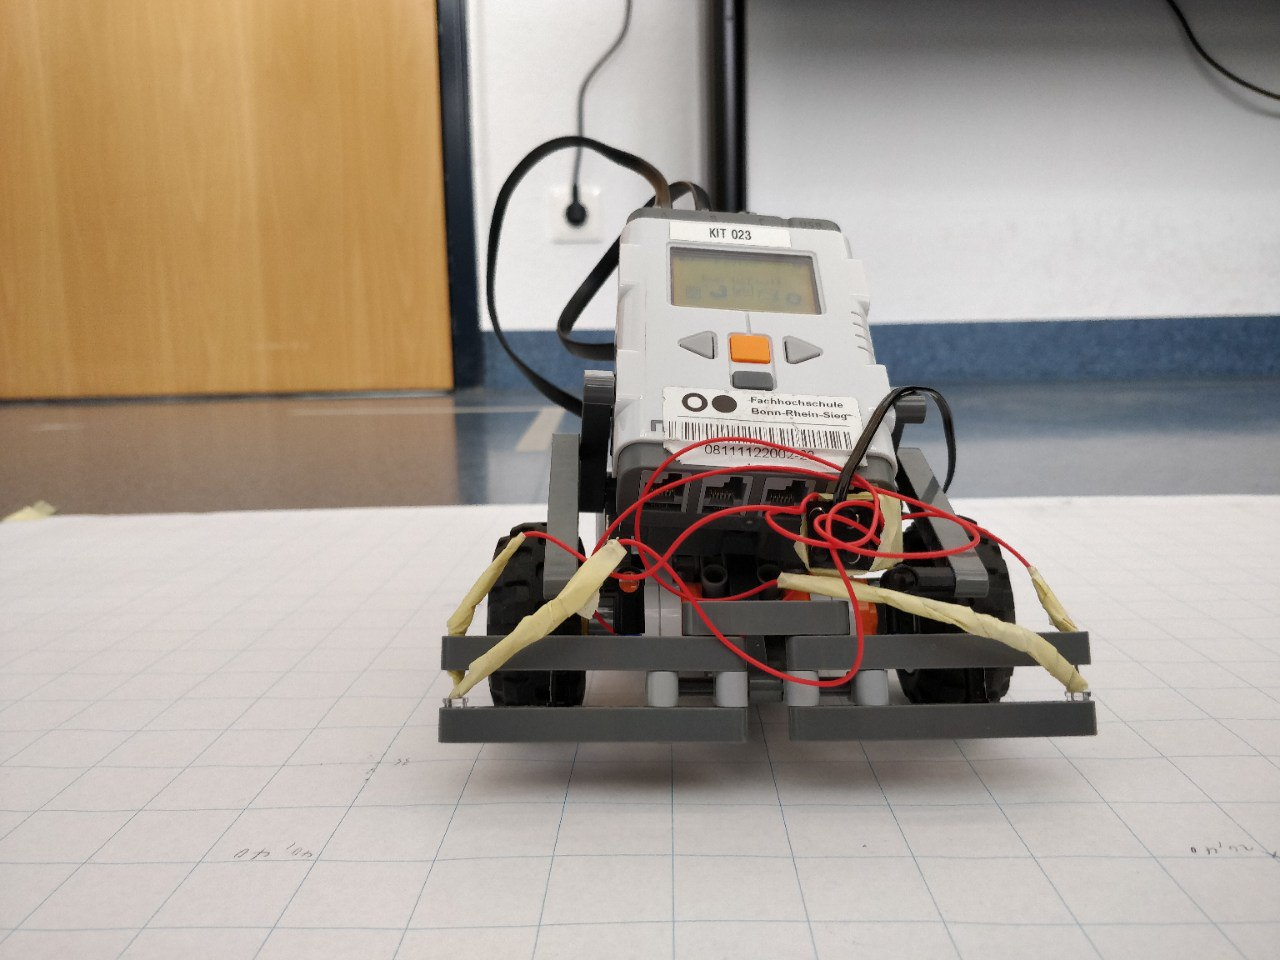
\includegraphics[width=.9\textwidth]{rf.jpg}
    \captionsetup{labelformat=empty}
    \caption{Front view} 
    \vspace{4ex}
  \end{minipage}%%
  \begin{minipage}[b]{0.3\textwidth}
    \centering
    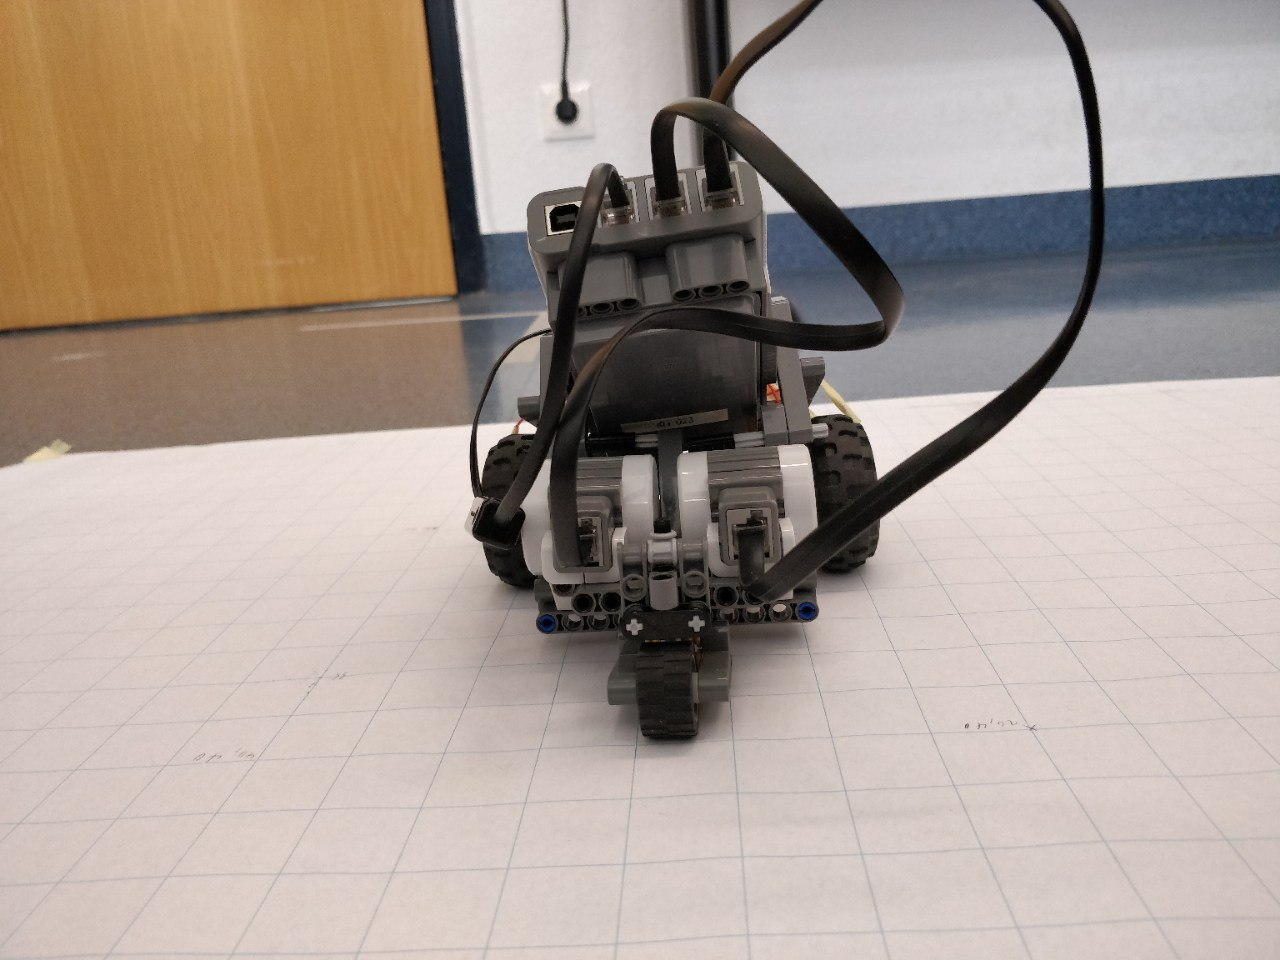
\includegraphics[width=.9\textwidth]{rb.jpg}
    \captionsetup{labelformat=empty}
    \caption{Back view} 
    \vspace{4ex}
  \end{minipage} 
  \begin{minipage}[b]{0.3\textwidth}
    \centering
    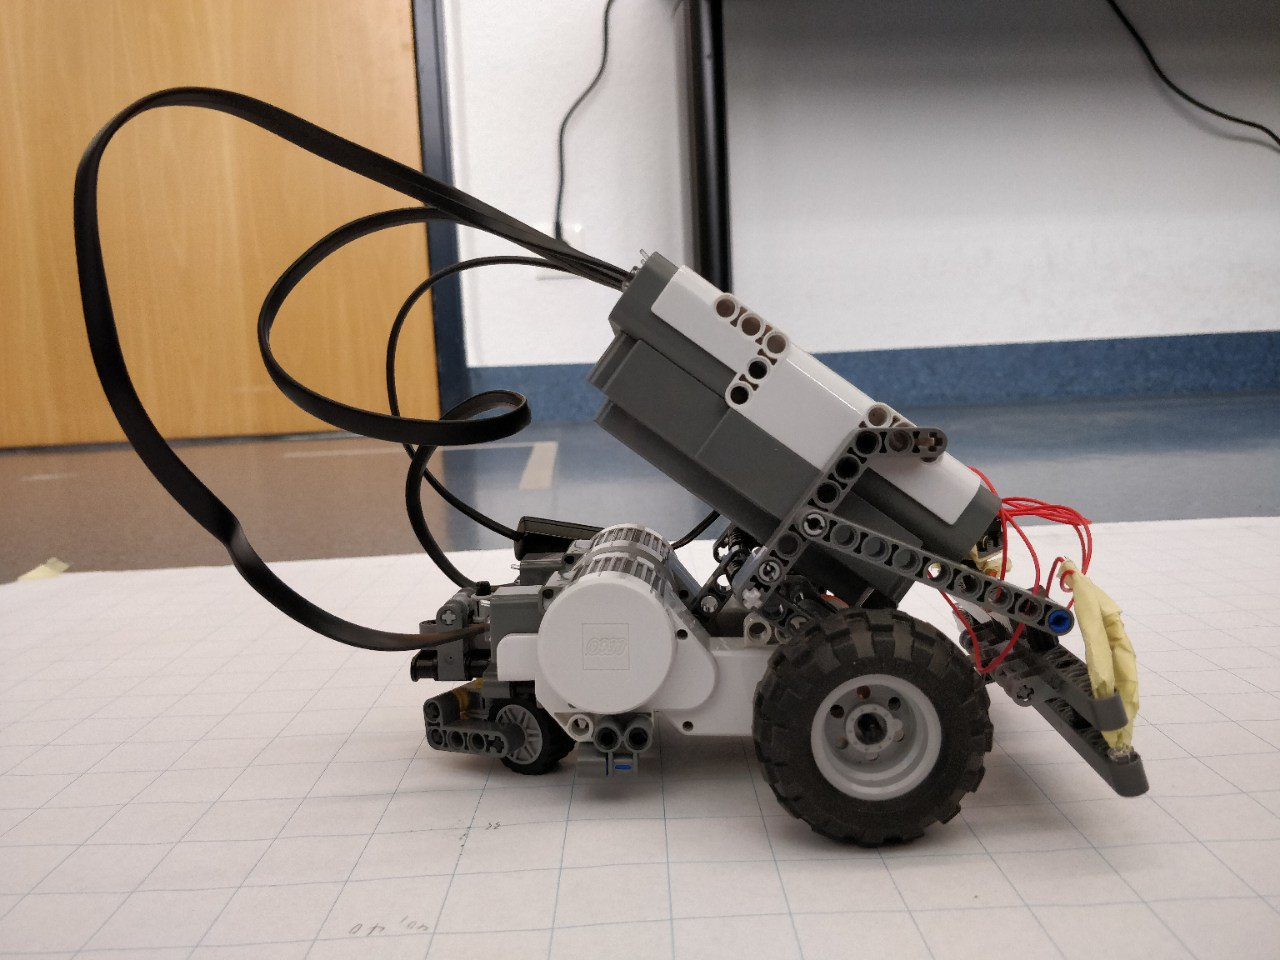
\includegraphics[width=.9\textwidth]{rr.jpg}
    \captionsetup{labelformat=empty}
    \caption{Right side view} 
    \vspace{4ex}
  \end{minipage}%% 
\newline
  \begin{minipage}[b]{0.3\textwidth}
    \centering
    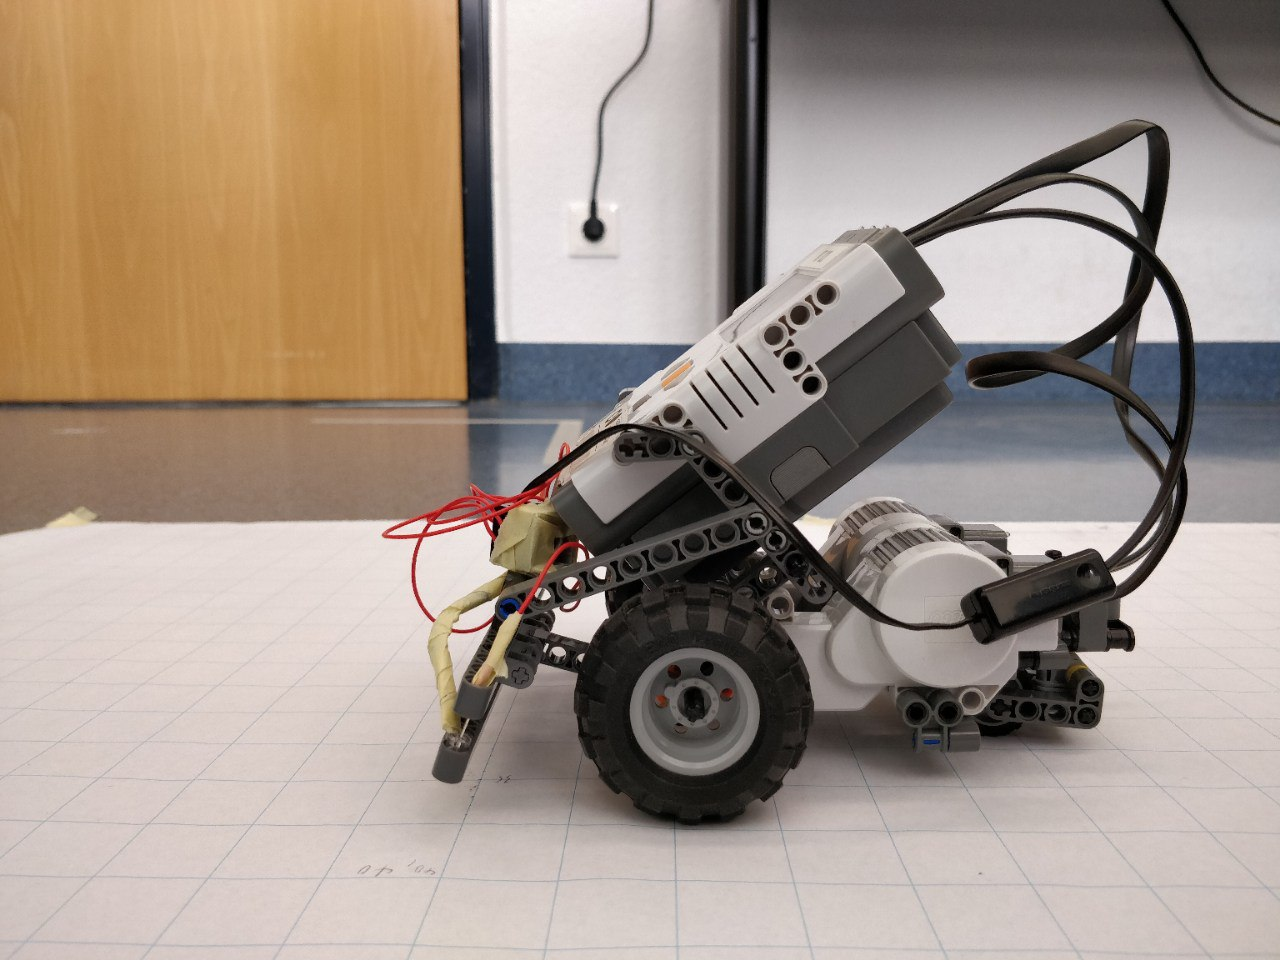
\includegraphics[width=.9\textwidth]{rl.jpg}
    \captionsetup{labelformat=empty}
    \caption{Left side view} 
    \vspace{4ex}
  \end{minipage}
  \begin{minipage}[b]{0.3\textwidth}
	\centering
	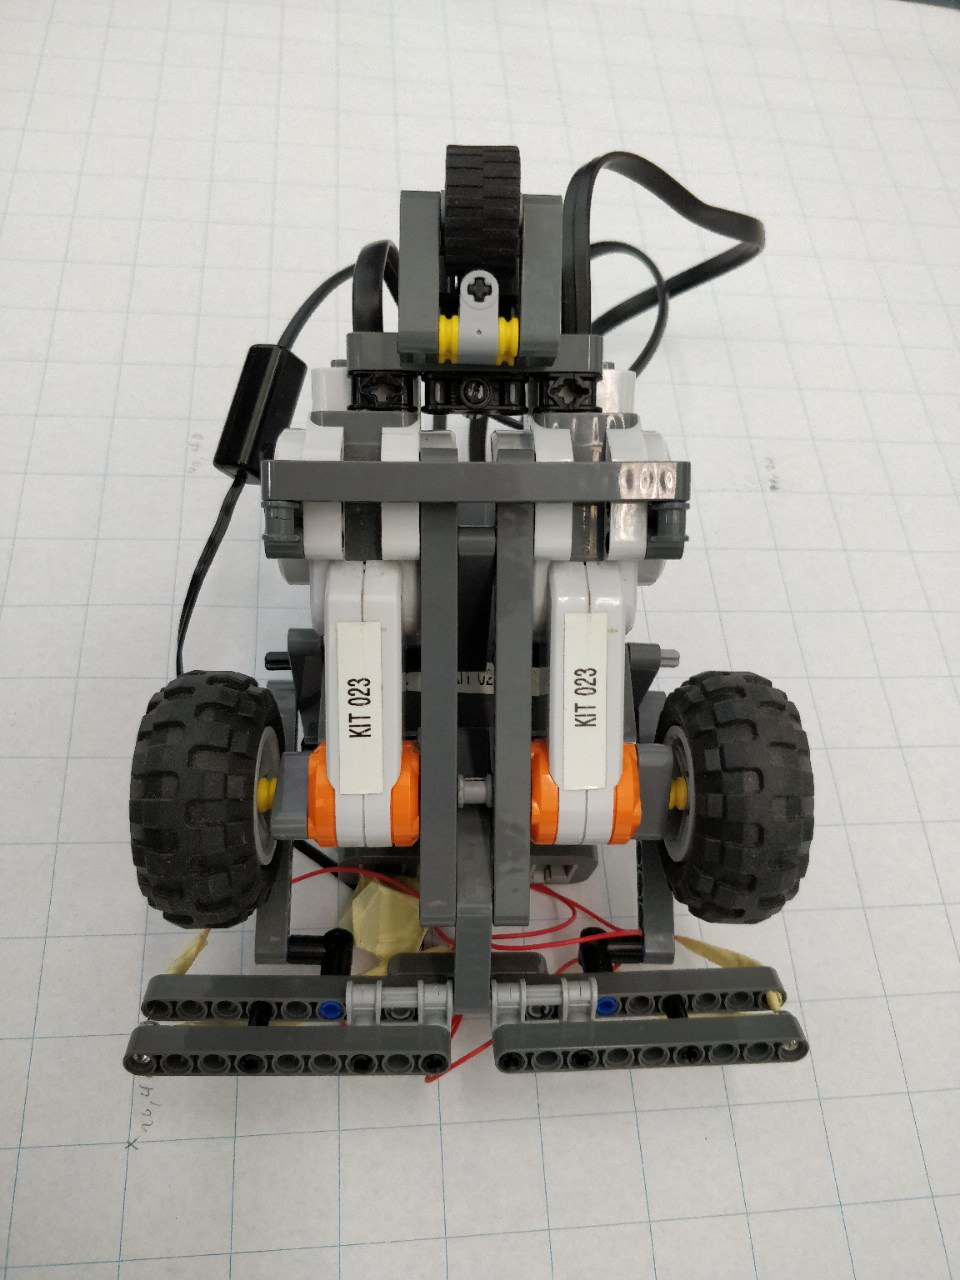
\includegraphics[width=.7\textwidth]{ru.jpg}
	\captionsetup{labelformat=empty}
	\caption{Bottom side view} 
	\vspace{4ex}
\end{minipage}%% 
\begin{minipage}[b]{0.3\textwidth}
	\centering
	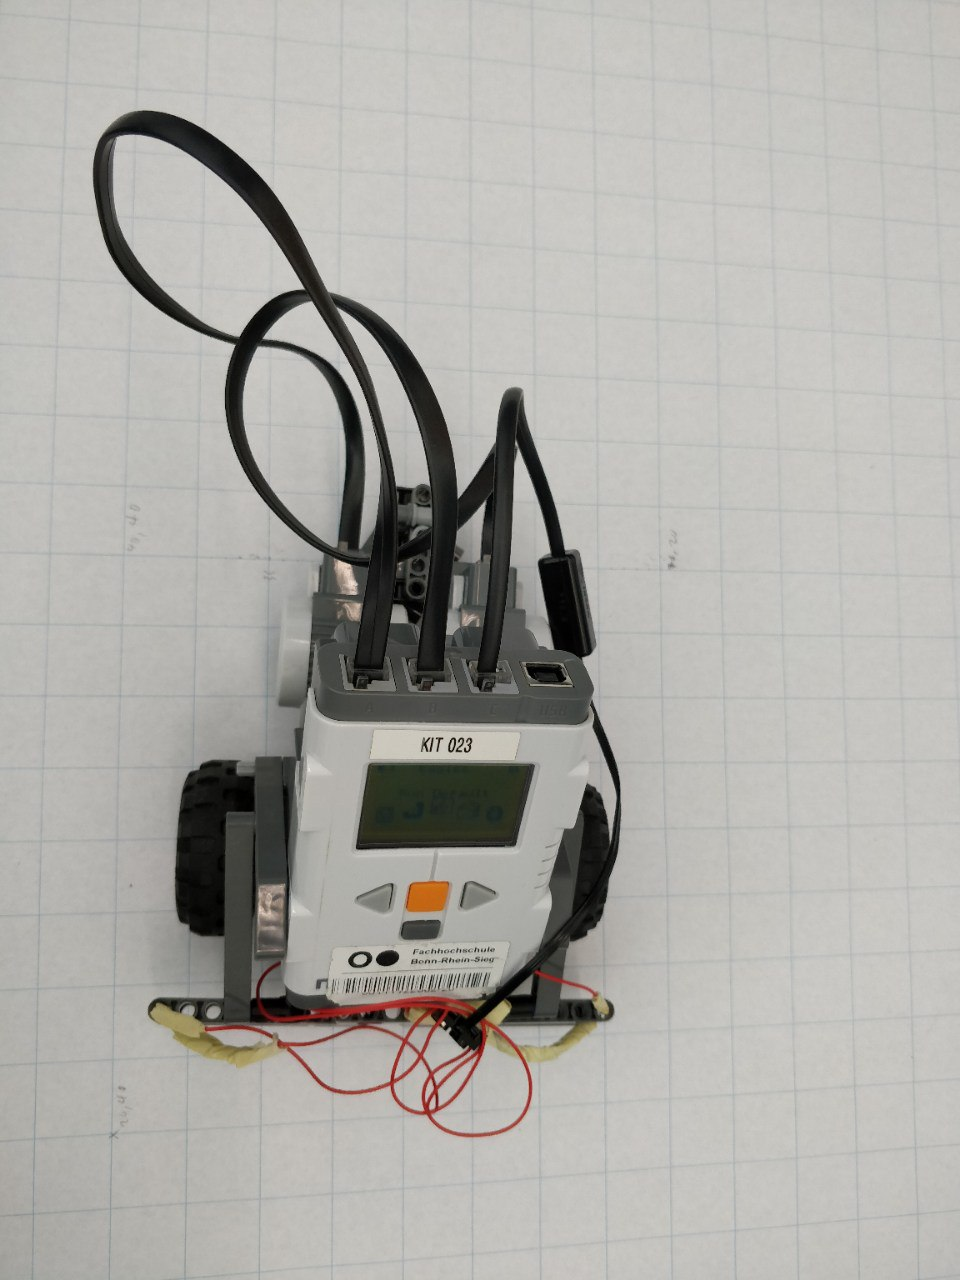
\includegraphics[width=.7\textwidth]{ro.jpg}
	\captionsetup{labelformat=empty}
	\caption{Top side view} 
	\vspace{4ex}
\end{minipage}
\caption{Lego robot design}
\label{legobot}
\end{figure}

%\begin{figure}[ht]
%\begin{center}
%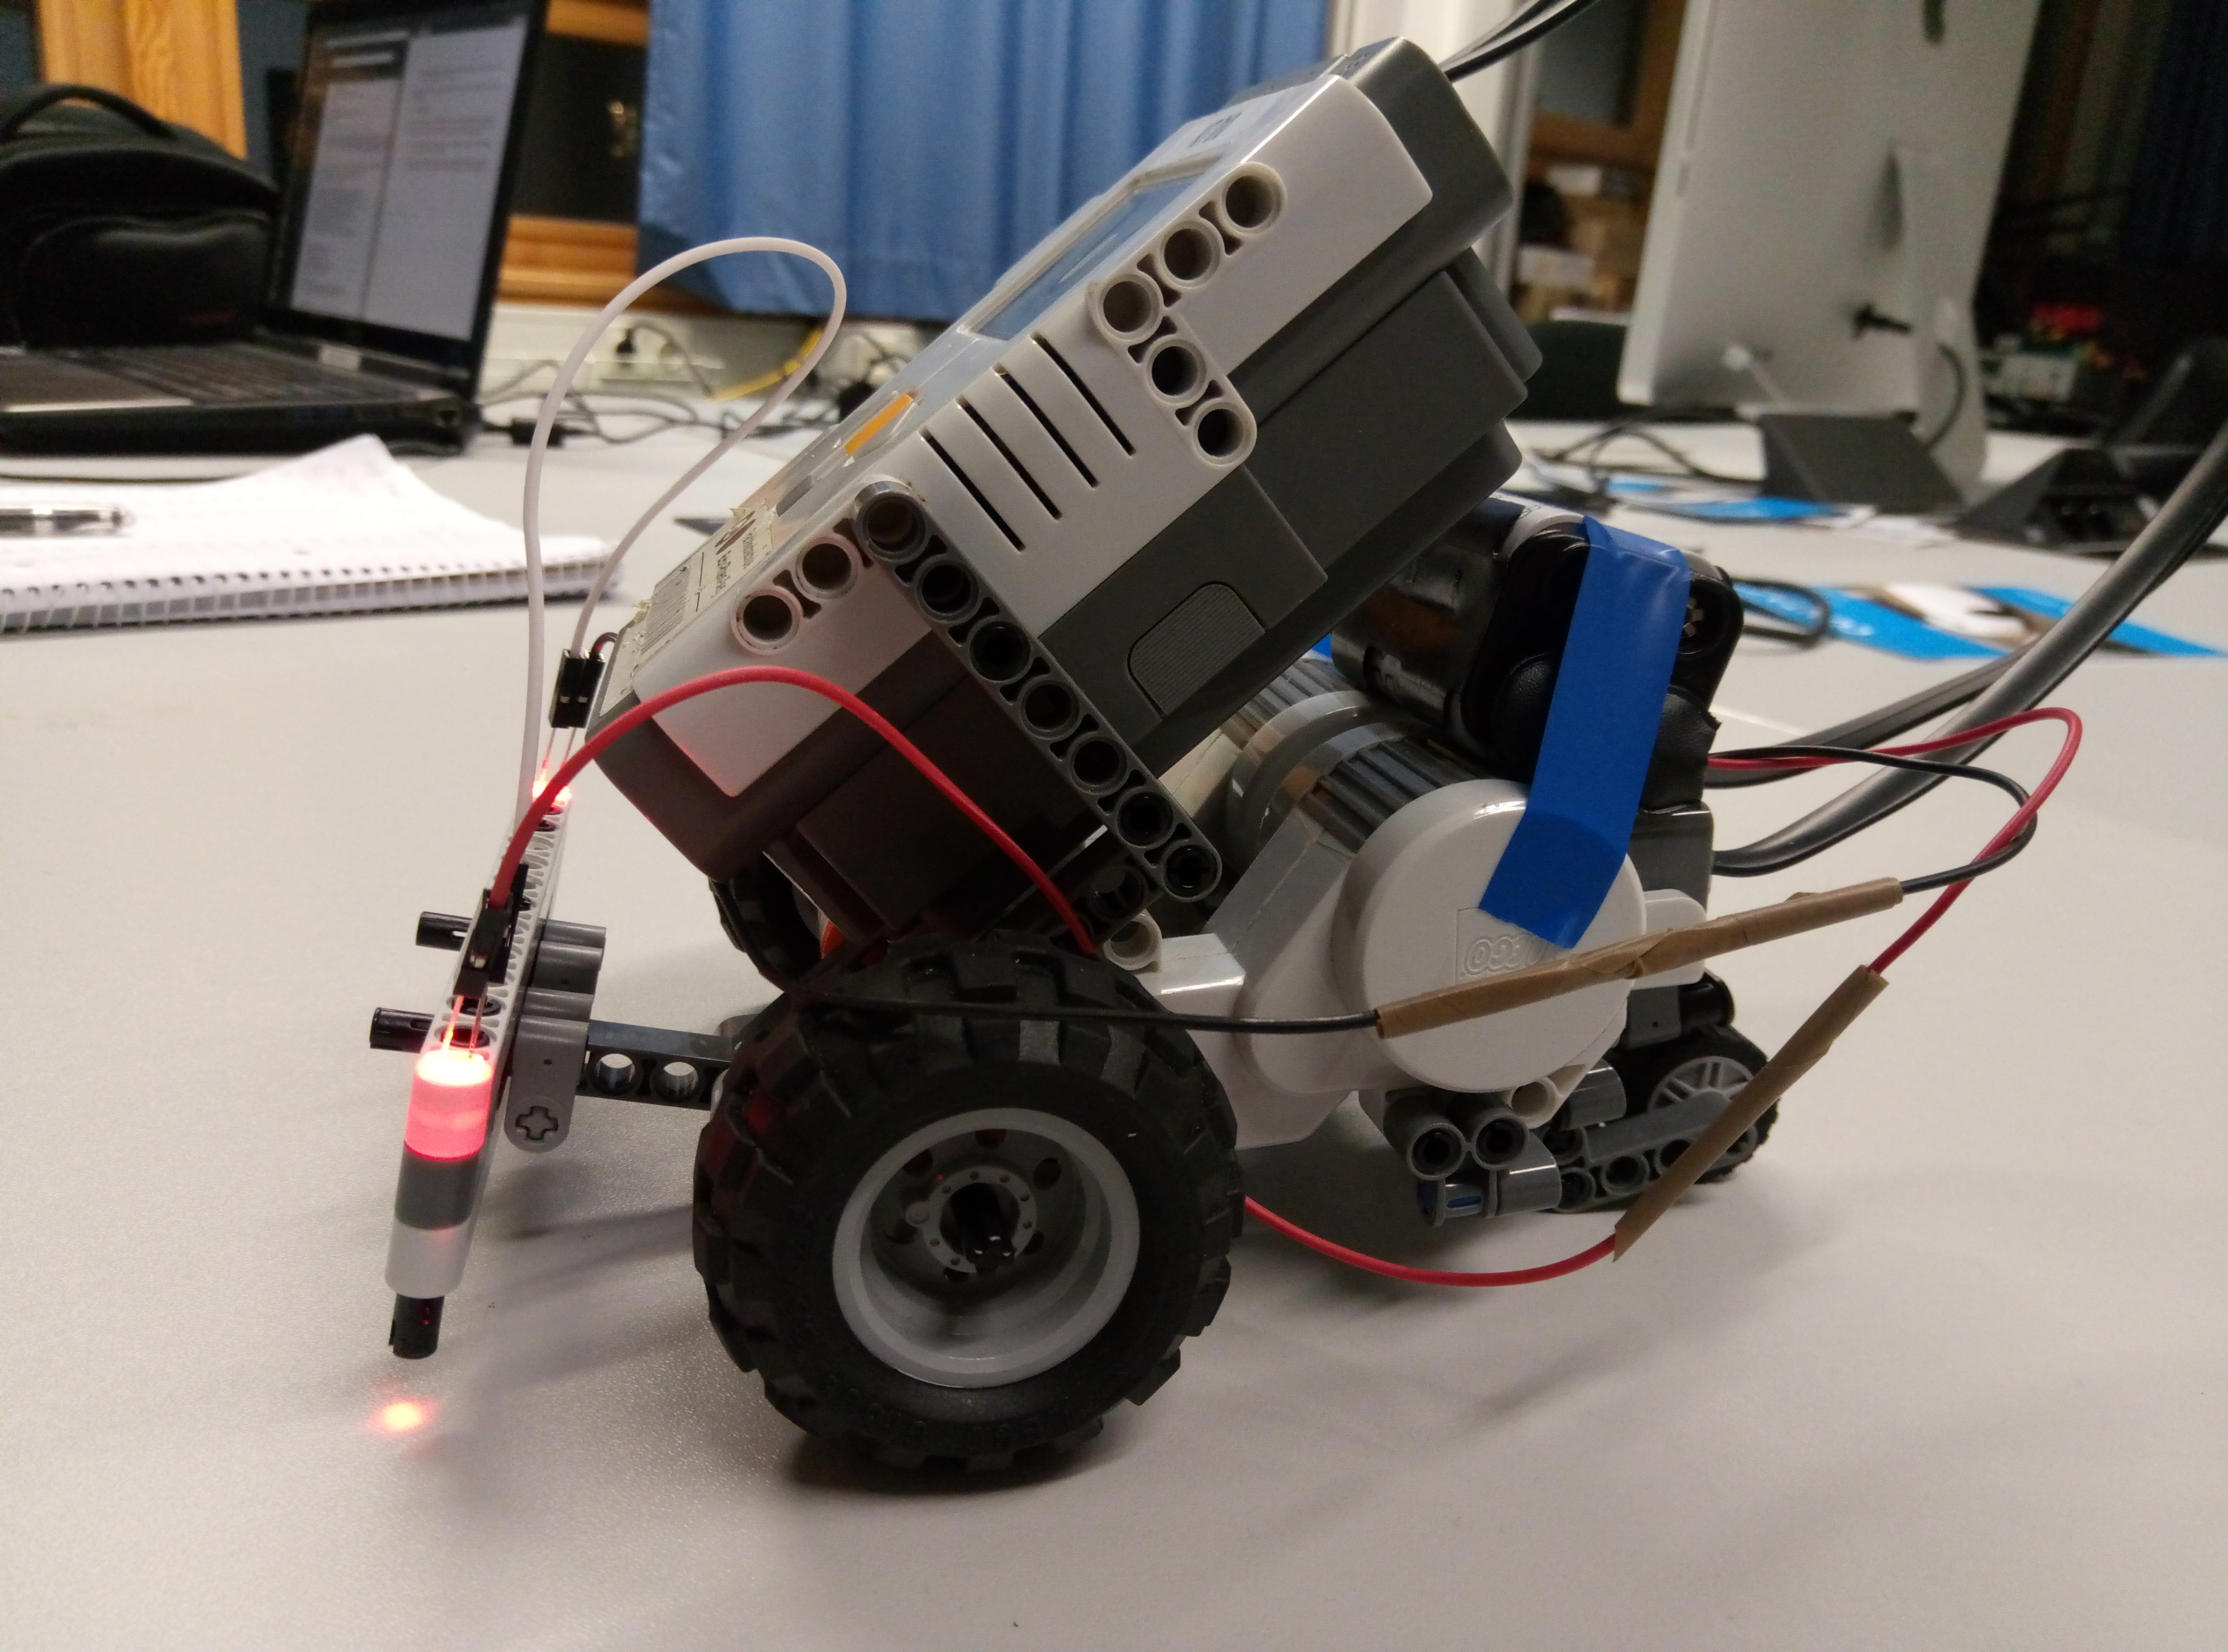
\includegraphics[width=0.7\textwidth]{lego_bot.jpg}
%\caption{Differential drive Lego bot with LEDs as measurement facility.}
%\label{legobot}
%\end{center}
%\end{figure}

\item We mounted two LEDs in front in order to measure the robots initial and final pose. We will mark center of LEDs with pen/pencil on the graph sheet as initial and final position of the Lego bot. There would be measurement error caused by hand marking the center of LEDs (which is not precise) on the graph paper.

\item The accuracy of the position marker measurement due to unresolved LED center resolution should be within 2-3mm.
\end{enumerate}

\subsection*{3. Deliverables 1.1}
\subsubsection*{Experimental setup}
\begin{itemize}
\item \textbf{Measurement system}: Our measurement system would consist of robot placed on a paper sheet as floor. We will attach two LEDs pointed towards floor near wheels which would give reference for start and end position. Current position of wheels will be the projection of light from led on the floor. We will fix the start position at beginning of the experiment which will be invariant for all trials. \textit{Expected End Position}, which will be calculated analytically, will be marked on the floor at beginning of the experiment as well. Robot's actual end position will be marked under the led focus. If necessary, additional arrangement of spacer tubes will be made to focus the light from LEDs. 

\item \textbf{Measurand}: Measurand in this experiment will be co-ordinates of each wheel's end position. 

\item \textbf{Measured quantity}: The variable to be measured is linear and angular deviation of end position of the wheels from expected end position. 
\begin{itemize}
	\item Linear Deviation of wheel 1 : 
	$$\delta x_{w1} = x_{w1}' - x_{w1}$$
	$$\delta y_{w1} = y_{w1}' - y_{w1}$$
	\item Linear Deviation of wheel 2 : 
	$$\delta x_{w2} = x_{w2}' - x_{w2}$$
	$$\delta y_{w2} = y_{w2}' - y_{w2}$$
	\item Mean Linear Deviation :  
	$$\delta x_{m} = x_{m}' - x_{m}$$
	$$\delta y_{m} = y_{m}' - y_{m}$$
	\item Angular Deviation (Angle between two lines joining expected wheel position and experimental wheel positions) : 
	$$\delta \theta = tan^{-1}\frac{\delta x_{m}}{\delta y_{m}}$$
\end{itemize}
\end{itemize}

\subsubsection*{Expected problems}
\begin{itemize}
\item \textbf{Systematic errors}\footnote{Partial explanation of systematic error is derived from \href{http://www-personal.umich.edu/~johannb/Papers/paper59.pdf}{http://www-personal.umich.edu/$\sim$johannb/Papers/paper59.pdf}.}: Systematic errors are caused by difference in the theoretical model and actual design of the robot such as, in our case, unequal wheel diameters ($E_D$) and uncertainty about effective wheelbase($E_B$) would create a systematic error in expected distance travelled (theoretical model, $\delta_{\text{trans-th}}$) and actual distance travelled ($\delta_{\text{trans}}$). These errors are robot specific don't change for a robot. Thus these errors can be improved upon by measuring their individual contributions and counter-acting their effects in software.\\
The error in wheel diameter can be defined as ratio between two wheel diameters,
\begin{align*}
E_D = \frac{D_R}{D_L}
\end{align*}
where $D_R$ and $D_L$ are actual right and left wheel diameters respectively. Error in wheel diameter affects the straight line motion whereas error in wheelbase affects the turning of the robot. The error in wheelbase is given as,
\begin{align*}
E_B = \frac{b_{\text{actual}}}{b_{\text{assumed}}}
\end{align*}
where $b_{\text{actual}}$ is the actual length of wheelbase and $b_{\text{assumed}}$ is the length of wheelbase assumed by software.
\item \textbf{Random errors}: Random errors are caused by inability of the sensors to measure the input beyond certain resolution. In our case inability to resolve current supplied beyond certain resolution would result in slight deviations in torques torques generated in motor which results in wheel rotation and ultimately results in variations in distance travelled by robot. We can correct this error by repeating the experiment multiple number of times and taking the mean value of the measurements. The mean value of change of pose can be given as,
\begin{align*}
\overline{\delta x} = \frac{1}{20} \sum_{i=1}^{20} \delta x_i \\
\overline{\delta y} = \frac{1}{20} \sum_{i=1}^{20} \delta y_i \\
\overline{\delta \theta} = \frac{1}{20} \sum_{i=1}^{20} \delta \theta_i
\end{align*}
The standard error of the mean for each variable is given by,
\begin{align*}
\hat{\sigma}_{\overline{\delta x}} = \sqrt{\frac{\sum_{i=1}^{20} (\delta x - \overline{\delta x})^2}{19 * 20}} \\
\hat{\sigma}_{\overline{\delta y}} = \sqrt{\frac{\sum_{i=1}^{20} (\delta y - \overline{\delta y})^2}{19 * 20}} \\
\hat{\sigma}_{\overline{\delta \theta}} = \sqrt{\frac{\sum_{i=1}^{20} (\delta \theta - \overline{\delta \theta})^2}{19 * 20}}
\end{align*}

\item \textbf{Measurement errors}: Errors may occur while marking the positions of the LED centres due to human error. Another possibility of human error while measuring the co-ordinates of the end position of wheels.   

\end{itemize}


\subsubsection*{Expected performance}
\begin{itemize}
\item We would need to remove the systematic error caused by the mismatch between actual robot design and the robot motion model by subtracting the effective offset. However the effective offset resolution will be determined by the random and measurement error.
\item The uncertainty in pose due to random errors for each trial can be given as,
\begin{align*}
\delta x = \delta x_{\text{measured}} \pm \hat{\sigma}_{\overline{\delta x}} \\
\delta y = \delta y_{\text{measured}} \pm \hat{\sigma}_{\overline{\delta y}} \\
\delta \theta = \delta \theta_{\text{measured}} \pm \hat{\sigma}_{\overline{\delta \theta}}
\end{align*}
\item The accuracy of the position marker measurement due to unresolved LED center resolution should be within 1-2 mm.
\end{itemize}

%%%%%%%%%%%%%%%%%%%%%%%%%%%%%%%%%%%%%%%%%%%%%%%%%%%%%%%%%%%%%%%%%%%%%%%%%%%%%
\end{document}